\documentclass[11pt]{article}
\usepackage{graphicx}
\usepackage{amssymb}
\usepackage{epstopdf}
\usepackage{amsfonts}
\usepackage{natbib}
\usepackage{subfigure}
\usepackage{pdfsync}
\usepackage{xspace}
\usepackage{xcolor}
\usepackage{tikz}
\usetikzlibrary{shapes.geometric, arrows}

\newcommand{\kid}{\mathrm{kid}}
\newcommand{\ma}{\mathrm{ma}}
\newcommand{\pa}{\mathrm{pa}}
\newcommand{\allelezero}{\tikz\draw[black,fill=white] (0,0) circle (0.8ex);}
\newcommand{\alleleone}{\tikz\draw[black,fill=black] (0,0) circle (0.8ex);}

\DeclareGraphicsRule{.tif}{png}{.png}{`convert #1 `dirname #1`/`basename #1 .tif`.png}


%% some handy things for making bold math
\def\bm#1{\mathpalette\bmstyle{#1}}
\def\bmstyle#1#2{\mbox{\boldmath$#1#2$}}
\newcommand{\thh}{^\mathrm{th}}


%% Some pretty etc.'s, etc...
\newcommand{\cf}{{\em cf.}\xspace }
\newcommand{\eg}{{\em e.g.},\xspace }
\newcommand{\ie}{{\em i.e.},\xspace }
\newcommand{\etal}{{\em et al.}\ }
\newcommand{\etc}{{\em etc.}\@\xspace}



%% the page dimensions from TeXShop's default---very nice
\textwidth = 6.5 in
\textheight = 9 in
\oddsidemargin = 0.0 in
\evensidemargin = 0.0 in
\topmargin = 0.0 in
\headheight = 0.0 in
\headsep = 0.0 in
\parskip = 0.2in
\parindent = 0.0in

% here are some tikz definitions
\tikzstyle{pa} = [rectangle, minimum width=0.93cm, minimum height=0.93cm,text centered, draw=black, fill=white]
\tikzstyle{ma} = [circle, minimum width=1cm, text centered, draw=black, fill=white]
\tikzstyle{opa} = [rectangle, minimum width=0.93cm, minimum height=0.93cm, text centered, draw=black, fill=lightgray]
\tikzstyle{oma} = [circle, minimum width=1cm, text centered, draw=black, fill=lightgray]

\tikzstyle{bpa} = [rectangle, minimum width=0.93cm, minimum height=0.93cm, text centered, draw=black, fill=blue!40]
\tikzstyle{bma} = [circle, minimum width=1cm, text centered, draw=black, fill=blue!40]
\tikzstyle{rma} = [circle, minimum width=1cm, text centered, draw=black, fill=red!40]


\tikzstyle{snode} = [circle, minimum width=0.45cm, text centered, draw=black, fill=white] % small node

\tikzstyle{arrow} = [thick,->,>=stealth]



\title{Applications of Graphs in Statistical \\
and Probabilistic Inference}
\author{Eric C. Anderson\thanks{
    Fisheries Ecology Division, 
    Southwest Fisheries Science Center, 
    110 Shaffer Road,
    Santa Cruz, CA 95060}
}
\begin{document}

\maketitle

\begin{abstract}
This is a brief narrative that follows, roughly, my guest lecture to
UCSC Math 115: Graph Theory, taught by Richard Montgomery, Winter 2016.
\end{abstract}

While this course will have steeped the students in the theoretical and algebraic
aspects of graph theory, I will be providing a look into some applications of
graphs in statistics and probability.

I enjoy talking about these
applications of graph theory because it is not immediately 
obvious how graphs and probability might mix.  
By this, I mean that many engineering applications of graphs involve situations where the graphical
representation is quite transparently a representation of a physical thing---for example
paths between points that must be traversed by a traveling salesman (with the edge weights
being distances), or routes upon which wire might be laid to provide an efficiently designed
telephone network.  In statistics, graphs are used to represent joint probability distributions
and glean properties of those distributions on a local and a global scale.  This is a little more
abstract. 

I am going to motivate this whole lecture with the example problem of computing probabilites of
genetic data on pedigrees.  We will consider just the simplest version of this problem---one genetic
locus with two alleles, keeping in mind that things can get very hairy with multiple linked markers. 
We focus on pedigrees for a few reasons: 1) part of my own research currently involves the application of 
algorithms on graphs to infer unknown pedigrees using genetic data sampled from wild populations 
(of fish, birds, whales, you name it\ldots); 2) the graphical structure of the problem follows the 
the lines of descent from parents to offspring, so it is somewhat tangible (it isn't
a telephone wire network, but it is still somewhat tangible\ldots); and 3) because the use
of directed graphs in statistics
has its origins in work on ``path diagrams" by the famed geneticist Sewall Wright in the mid-1900's.

It is important to keep in mind, however, that these graphical concepts apply to probabilistic models
and statistical inference much more widely than just to pedigrees.  In fact, their general utility 
in statistics began to be widely appreciated in the 1970's and it became clear that similar 
notions were in use in a wide variety of fields from statistical physics, to electrical engineering
and computer science.  In fact, one of the wonderful benefits of thinking about probability distributions
in terms of graphs is that it has made it much easier for researchers in a wide variety of fields to
appreciate just how similar many of the problems that they work on are, in terms of their 
essential probabilistic assumptions and calculations.  

\section{Overview}

The lecture today will break down into the following sections:
\begin{itemize}
\item introduction to necessary genetics and probabilities and the idea of inference of genotypic state,
\item the {\em acyclic directed} graphical model formalism and factorization into conditional probabilities,
\item conditional independence and the {\em undirected graphical} model formalism, moralization, 
neighborhoods.  ({\sl Much, much more could be said here about Markov random fields, 
factorization over maximal clique potentials,
graphical assessment of the computational complexity of inference, the treewidth of a graph,
etc. but we will skip most of that.})
\item the {\em factor-graph} model formalism, the sum-product algorithm, and loopy belief propagation,
\item pedigree inference.
\end{itemize}
This list of topics, treated in depth, could easily require a full quarter, so we will just be
skimming the
surface here. But what I hope that people will take home from this is an appreciation 
of the three different ways of representing probability distributions, graphically, and some of their
applications, and the utility of graphical representations for algorithm development.


\section{Simple Genetics and Probability}
\subsection{Basic genetics}
With today's genetic technologies we can find a specific location in an individual's genome and read the DNA base 
(an A, C, G, or T) at exactly the same spot on a chromosome within or across individuals.
Such a location is called a ``locus'' or a ``SNP marker'' and the specific base that is found there
is called an {\em allele}. In a {\em diploid} there are two copies of the genome 
(one from the mother and one from the father) in an individual, which means that his/her {\em genotype}
at the locus has two {\em allelic} values, like AA, or AG, or TT, \etc  
We typically do not know which copy came from the
mother or the father, so we take the two allelic values in the genotype as {\em unordered}.  

At most SNP markers, only two of the possible four DNA bases will be seen amongst all individuals in the 
population, thus, we can call one of the alleles \allelezero{} and the other one \alleleone{},  and
refer to the genotype as the number of \alleleone{} alleles in the genotype.  Thus genotypes can be 0, 1, or 2.  For example, 
if we let \allelezero{} refer to the base  A and \alleleone{} refer to the base G, then the
diploid genotypes can be named as follows 
\begin{itemize}
\item AA = \allelezero\,\allelezero{} = 0
\item AG or GA =  \allelezero\,\alleleone{} or \alleleone\,\allelezero{} = 1
\item GG = \alleleone\,\alleleone{} = 2
\end{itemize}
If you were to grab an individual from a population, the probability of his genotype, $Y$,
can be determined by the frequency of the alleles in the population.  Let $q$ be 
the relative frequency of the \alleleone{} allele.  Then the genotype frequencies (assuming that 
they are drawn, independently, from the population into the individual) are
\begin{eqnarray*}
P(Y = 0) & = & (1-q)^2 \\
P(Y = 1) & = & 2q(1-q) \\
P(Y = 2) & = & q^2 \\
\end{eqnarray*}

\subsection{Mendelian inheritance and conditional probabilities}
Gregor Mendel (a monk in the 1800's with a penchant for growing and breeding pea plants, sipping tea,
making observations, and thinking deeply about them) 
showed that when a diploid mother and father produce a child, each parent passes only one copy
of a locus to its child.  The copy that gets passed on is chosen randomly (probability $\frac{1}{2}$)
within each parent and is independent of the copy that gets passed on by the other parent.

We can draw a picture of the production of an offspring like so:
\begin{center}
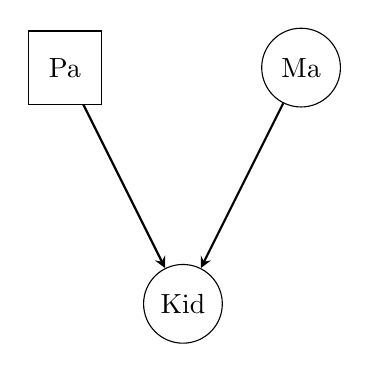
\begin{tikzpicture}[node distance=3cm]

\node (pa) [pa] {Pa};
\node (ma) [ma, right of=pa] {Ma};
\node (kid) [ma, yshift= -3.0cm, xshift=1.5cm] {Kid};

\draw [arrow] (pa) -- (kid);
\draw [arrow] (ma) -- (kid);
\end{tikzpicture}
\end{center}
This is a simple pedigree.  Males are represented as squares and females as circles
and lines of descent are depicted by directed edges.  You might
also recognize it as directed graph that has no directed cycles.

A natural thing to think about in this case is the {\em conditional probability} of $\mathrm{Kid}$'s genotype
given the genotypes of its parents, \ie $P(Y_\kid | Y_\pa, Y_\ma)$.  These probabilities are
easily worked out from Mendel's laws.  There are $3^3 = 27$ such conditional probabilities.  Below are
9 of them for the case where $Y_\pa = 1$, \ie  \allelezero\,\alleleone{}.

{
\renewcommand{\baselinestretch}{1.57}
\large
\[
P(Y_\kid | Y_\pa = 1\;\allelezero\,\alleleone{}, Y_\ma) = \bordermatrix{ 
Y_\kid\downarrow ~ ~ Y_\ma\rightarrow &  0\;\allelezero\,\allelezero{} & 1\;\allelezero\,\alleleone{} & 2\;\alleleone\,\alleleone{} \cr
0\;\allelezero\,\allelezero{}  &  \frac{1}{2}   &  \frac{1}{4}   &  0  \cr
1\;\allelezero\,\alleleone{}   &  \frac{1}{2}   &  \frac{1}{2}   &  \frac{1}{2}  \cr
2\;\alleleone\,\alleleone{}    &     0          &  \frac{1}{4}   &  \frac{1}{2}  \cr
}
\]
}
\renewcommand{\baselinestretch}{1.00}


Wow! That is super simple.  We are just dealing with probabilities of 0, $\frac{1}{2}$, $\frac{1}{4}$; 
when does this get challenging?  That is the fun part of these sorts of problems---when you build
up lots of simple probabilities in a complex web of probabilistic dependence things can eventually get hairy.

\subsection{Observed variables, joint probability}
Here, let us introduce a little notational twist on the pedigree above: we will shade the
vertices that are observed.  In other words, in the pedigrees below the shading indicates we have observed whether
the genotype of each individual is 0, 1, or 2.  The pedigree on the right actually shows the observed genotypes.
\begin{center}
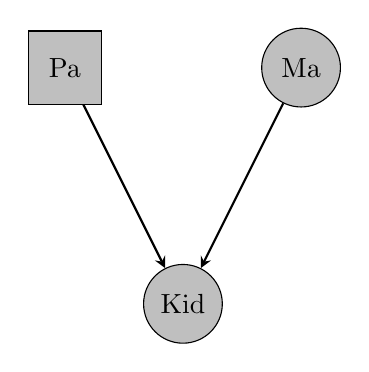
\begin{tikzpicture}[node distance=3cm]

\node (pa) [opa] {Pa};
\node (ma) [oma, right of=pa] {Ma};
\node (kid) [oma, yshift= -3.0cm, xshift=1.5cm] {Kid};

\draw [arrow] (pa) -- (kid);
\draw [arrow] (ma) -- (kid);
\end{tikzpicture}
~~~~~~~~~~~~~~~~~~~~~~~~~~~~
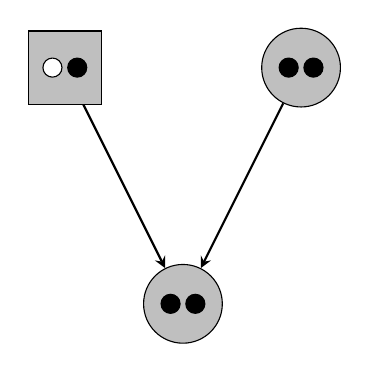
\begin{tikzpicture}[node distance=3cm]

\node (pa) [opa] {\allelezero\,\alleleone};
\node (ma) [oma, right of=pa] {\alleleone\,\alleleone};
\node (kid) [oma, yshift= -3.0cm, xshift=1.5cm] {\alleleone\,\alleleone};

\draw [arrow] (pa) -- (kid);
\draw [arrow] (ma) -- (kid);
\end{tikzpicture}
\end{center}

If you are a statistician, one of the things you will love to do is to calculate the probability
of all your observed data, as doing so forms the basis for using your data to learn about things
that you might not have observed---the process called {\em inference} (more on that later).  

In the right-hand pedigree above, the probability of all three individuals is a {\em joint}
probability, which simply means it is a probability of two or more things (\ie random variables),
considered together. We can write a joint probability like this $P(X_\pa = 1, X_\ma = 2, X_\kid = 2)$.
But how to compute it?  Well, you can think about how the data would have been generated:
\begin{enumerate}
\item First Pa must have genotype 1, and Ma must have genotype 2.  This happens with
probabilities $2q(1-q)$ and $q^2$.
If the parents' genotypes are independent (as they are) then the probability of both
is just their product.
\item Then those two parents must have a kid with a genotype of 2, which happens with 
probability $\frac{1}{2}$. 
\end{enumerate}
So,
\begin{eqnarray*}
P(X_\pa = 1, X_\ma = 2, X_\kid = 2) & = & P(X_\pa = 1) P(X_\ma = 2) P(X_\kid = 2 | X_\pa = 1, X_\ma = 2) \\
& = & 2q(1-q) \cdot q^2 \cdot \frac{1}{2}
\end{eqnarray*}

\subsection{Inference, a simple example}
Imagine that you have observed the genotype of Pa and Kid, but not Ma,
\begin{center}
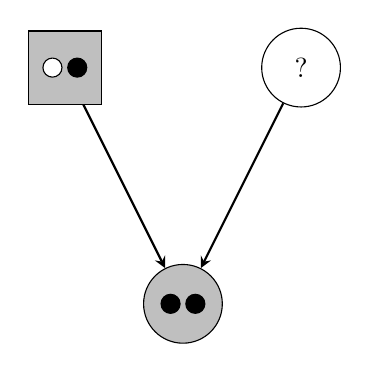
\begin{tikzpicture}[node distance=3cm]

\node (pa) [opa] {\allelezero\,\alleleone};
\node (ma) [ma, right of=pa] {?};
\node (kid) [oma, yshift= -3.0cm, xshift=1.5cm] {\alleleone\,\alleleone};

\draw [arrow] (pa) -- (kid);
\draw [arrow] (ma) -- (kid);
\end{tikzpicture}
\end{center}
\ldots so you would like to use all the information in the above figure to {\em infer} (as best you can)
the genotype of Ma.  We have two sources of information here:
\begin{enumerate}
\item If we never looked at Kid and Pa, but rather just plucked Ma out of the population we know that
the probability of her genotype would be $(1-q)^2$ if \allelezero\,\allelezero, $2q(1-q)$ if \allelezero\,\alleleone{} or
\alleleone\,\allelezero, or $q^2$ if $(1-q)^2$ if \alleleone\,\alleleone.
\item If we just focus on Ma's relationship with Kid and Pa, we can evaluate the evidence in favor
of Ma's genotype by the relative size of $P(Y_\kid = 2|Y_\pa = 1, Y_\ma)$ considered as a function
of $Y_\ma$.  This is sometimes called the ``likelihood.''
\end{enumerate}
These two pieces of evidence are combined together using {\em Bayes' law} to compute the posterior 
probability.  If $q=0.6$ then the posterior probability of Ma's genotype is 0 for 
\allelezero\,\allelezero, 0.4 for \alleleone\,\allelezero{} or \allelezero\,\alleleone, and 0.6 for
\alleleone\,\alleleone.  Left as an exercise if it is not already familiar to you.

Inference about an individual genotype in a pedigree (vertex in a graph) can be seen as a process
of computing probabilites for an unobserved genotype (vertex in a graph) given that information
from the observed genotypes (vertices in a graph) on the pedigree.  This has many uses in 
biology, ecology, medicine, \etc

\section{Acyclic directed graphs}
The pedigree above is an example of an {\em acyclic directed} graph, often called a DAG for
short.  The wonderful thing about DAGs: if you have a joint probability distribution that
factorizes into a {\em product of conditional probabilities}, you can represent the 
factorization of the distribution as a DAG.

In general, a joint distribution that factorizes according to a DAG with vertices $X_1,\ldots, X_K$  
representing random variables can be written as the product:
\[
P(X_1,\ldots, X_K) = \prod_{i=1}^K P(X_i | \mathrm{pa}(X_i))
\]
where $\mathrm{pa}(X_i)$ denotes the {\em parents} of $X_i$ in the DAG, and we
follow the convention that if $\mathrm{pa}(X_i) = \emptyset$ then 
$P(X_i | \mathrm{pa}(X_i)) = P(X_i)$---simply the ``prior'' probability of $X_i$.

For example, take a DAG that is not a pedigree:
\begin{center}
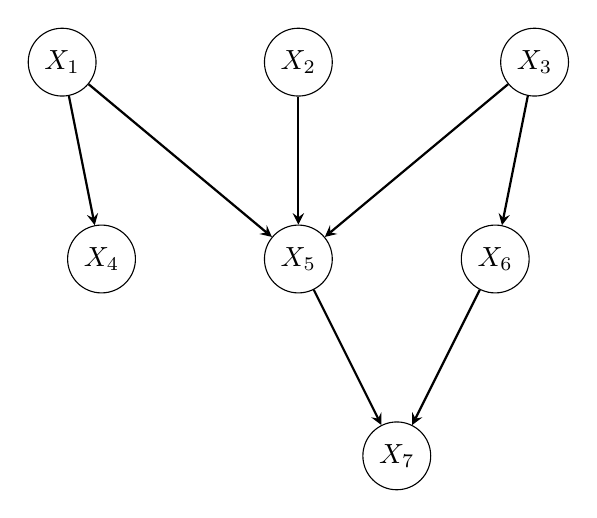
\begin{tikzpicture}[node distance=3cm]

\node (x1) [snode] {$X_1$};
\node (x2) [snode, right of=x1] {$X_2$};
\node (x3) [snode, right of=x2] {$X_3$};
\node (x4) [snode, yshift= -2.5cm, xshift=0.5cm] {$X_4$};
\node (x5) [snode, yshift= -2.5cm, xshift=3.0cm] {$X_5$};
\node (x6) [snode, yshift= -2.5cm, xshift=5.5cm] {$X_6$};
\node (x7) [snode, yshift= -5.0cm, xshift=4.25cm] {$X_7$};

\draw [arrow] (x1) -- (x4);
\draw [arrow] (x1) -- (x5);
\draw [arrow] (x2) -- (x5);
\draw [arrow] (x3) -- (x5);
\draw [arrow] (x3) -- (x6);
\draw [arrow] (x5) -- (x7);
\draw [arrow] (x6) -- (x7);
\end{tikzpicture}
\end{center}
Writing down the factorization of a distribution that respects the above graph is left
as an exercise.  It is worth noting that, though the above graph contains a cycle,
it is not a directed cycle, so it is still a DAG.

\subsection{What good are DAGs?}
This is a fair question.  It appears to me that the primary value of DAGs in the field of 
probabilistic graphical models is that they can be used to represent the factorization
of joint probability distributions into conditional probabilities.  This makes a very nice
way of visualizing the structure of complex probability models and especially of
{\em Bayesian hierarchical models}.  But beyond that, when it comes to tasks such 
as graphically assessing conditional independence, or designing algorithms for 
inference, other types of related graphs provide more suitable and useful representations.
We illustrate this with the example in the following section.

\subsection{Which relatives really matter?}
Let us consider the pedigree below and ask ourselves the question, ``If we want to do inference
on the genotype of individual $A$ given the observed genotypes of individuals
1--15, which of those observed individuals can we safely ignore and which must we include 
in our calculations?
\begin{center}
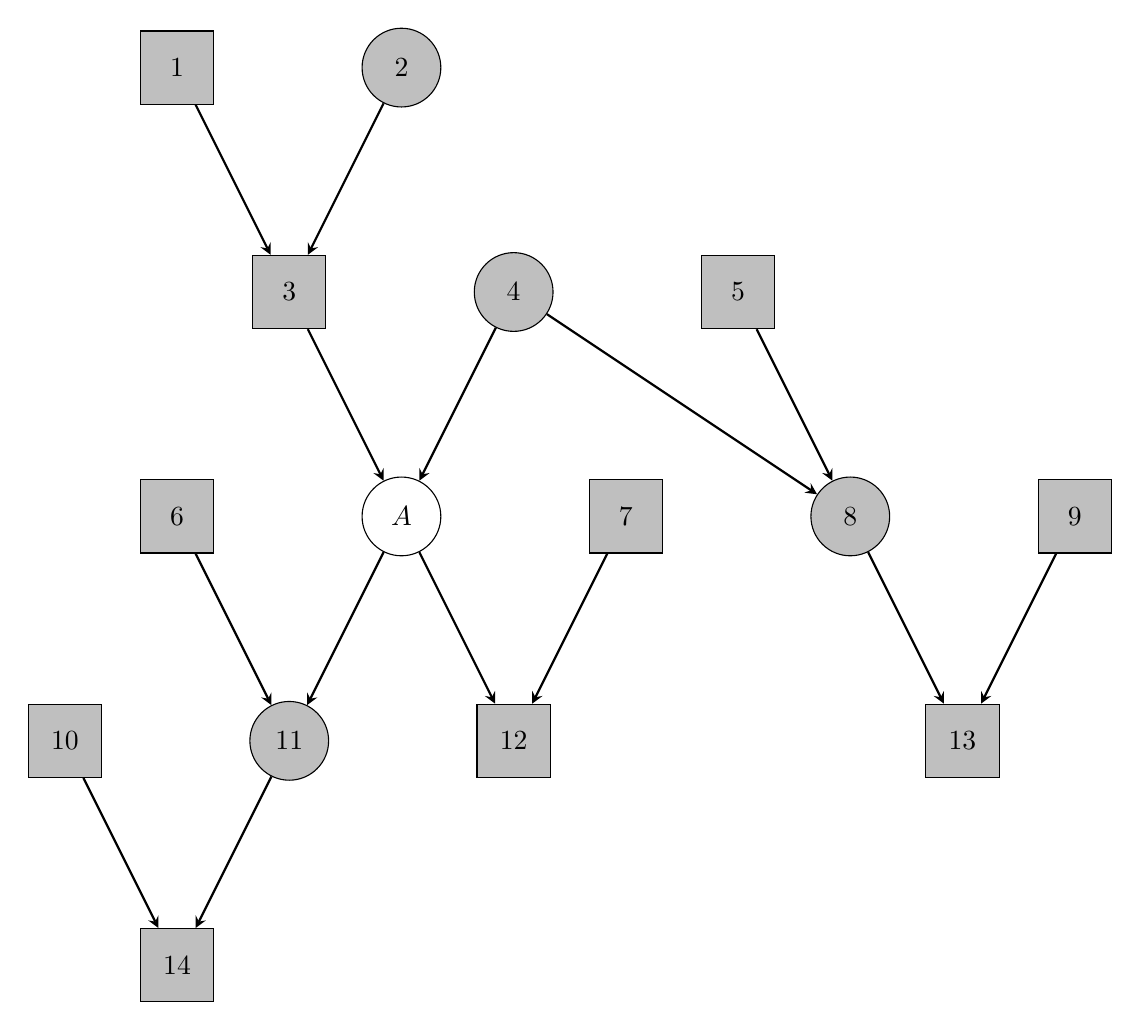
\begin{tikzpicture}[node distance=2.85cm]

\node (1) [opa] {1};
\node (2) [oma, right of=1] {2};

\node (3) [opa, below of=1, xshift=1.425cm] {3};
\node (4) [oma, right of=3] {4};
\node (5) [opa, right of=4] {5};

\node (6) [opa, below of=3, xshift=-1.425cm] {6};
\node (A) [ma, right of=6] {$A$};
\node (7) [opa, right of=A] {7};
\node (8) [oma, right of=7] {8};
\node (9) [opa, right of=8] {9};

\node (10) [opa, below of=6, xshift=-1.425cm] {10};
\node (11) [oma, right of=10] {11};
\node (12) [opa, right of=11] {12};
\node (13) [opa, right of=12, xshift=2.85cm] {13};

\node (14) [opa, below of=10, xshift=1.425cm] {14};

\draw [arrow] (1) -- (3);
\draw [arrow] (2) -- (3);

\draw [arrow] (3) -- (A);
\draw [arrow] (4) -- (A);
\draw [arrow] (4) -- (8);
\draw [arrow] (5) -- (8);

\draw [arrow] (6) -- (11);
\draw [arrow] (A) -- (11);
\draw [arrow] (A) -- (12);
\draw [arrow] (7) -- (12);
\draw [arrow] (8) -- (13);
\draw [arrow] (9) -- (13);

\draw [arrow] (10) -- (14);
\draw [arrow] (11) -- (14);

\end{tikzpicture}
\end{center}
When doing computation or statistics, being able to ignore {\em irrelevant} data is always
advantageous, but you don't want to toss out relevant data. So, some way of assessing 
which individual genotypes are relevant to inference of $A$'s genotype is in order.

It is relatively easy to figure this out from the factorized joint density---any variables 
that appear (on either side of the ``$|$'') in a conditional probability density with 
$Y_A$ are relevant. For example, the full joint probability of the pedigree above can be written:
\begin{eqnarray*}
P(\mathrm{all}) & = & P(Y_1)P(Y_2)P(Y_3|Y_1,Y_2)P(Y_4)P(Y_5) \\
  & \times  & P(Y_6)\textcolor{blue}{P(Y_A|Y_3,Y_4)}P(Y_7)P(Y_8|Y_4,Y_5)P(Y_9) \\
  & \times  & P(Y_{10})\textcolor{blue}{P(Y_{11}|Y_6,Y_A)P(Y_{12}|Y_A,Y_7)}P(Y_{13}|Y_8,Y_9) \\
  & \times  & P(Y_{14}|Y_{10},Y_{11})
\end{eqnarray*}
The only variables that can tell us something about $Y_A$ (at least if everything is 
observed except for $Y_A$) are those that are muddled up inside conditional probabilities
with $Y_A$ in the joint
probability.  They are \textcolor{blue}{$(Y_3, Y_4, Y_6, Y_7, Y_{11}, Y_{12})$}.

If you are excited about graphical representations of distributions you might like a
nice, tidy, graphical way of visualizing the relatives who matter, perhaps by {\em adjacency} 
in the graph. Alas! That doesn't work with this DAG (or, in general, any DAG).
Behold, below, that the
relevant relatives are not actually all adjacent to $A$ in the directed graph.
\begin{center}
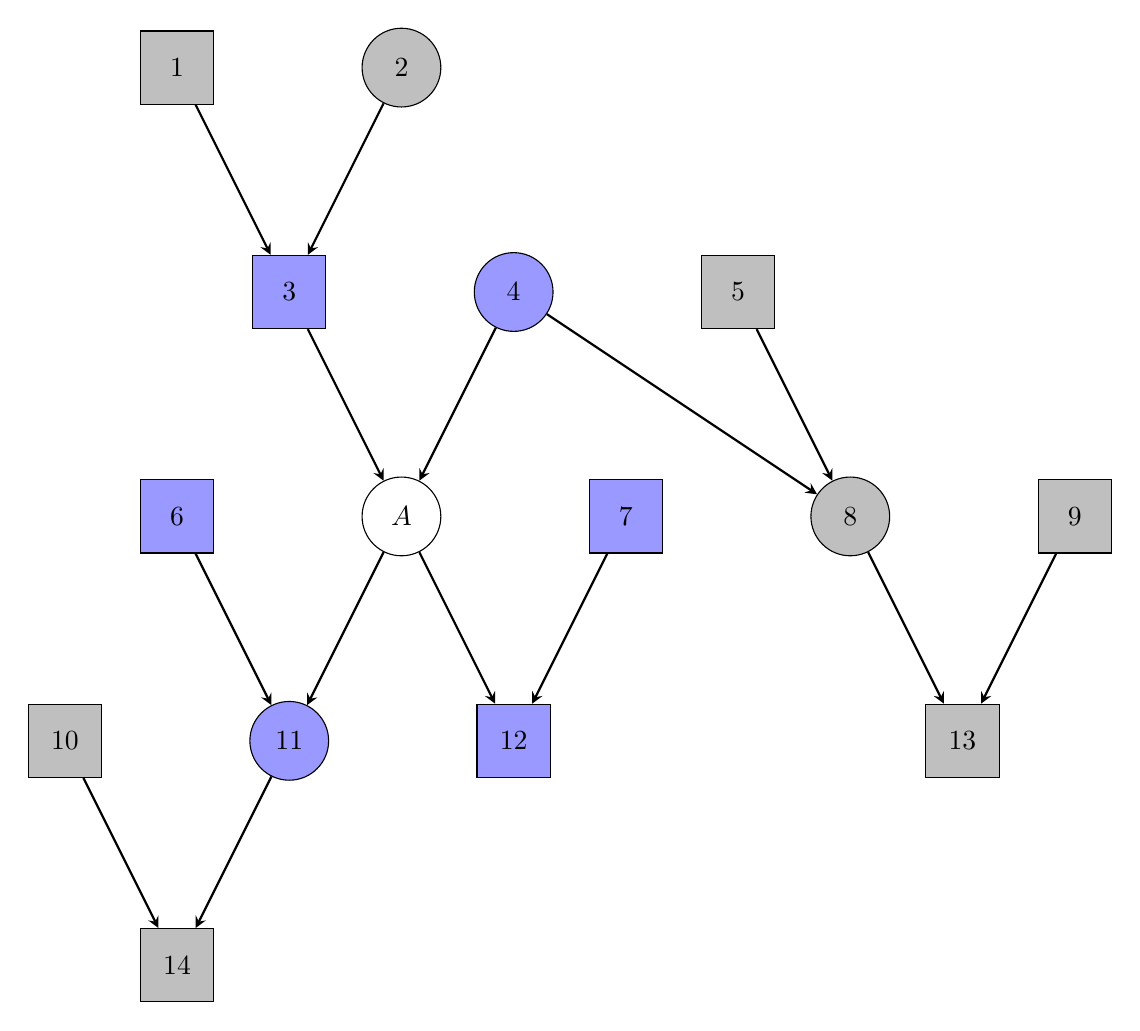
\begin{tikzpicture}[node distance=2.85cm]

\node (1) [opa] {1};
\node (2) [oma, right of=1] {2};

\node (3) [bpa, below of=1, xshift=1.425cm] {3};
\node (4) [bma, right of=3] {4};
\node (5) [opa, right of=4] {5};

\node (6) [bpa, below of=3, xshift=-1.425cm] {6};
\node (A) [ma, right of=6] {$A$};
\node (7) [bpa, right of=A] {7};
\node (8) [oma, right of=7] {8};
\node (9) [opa, right of=8] {9};

\node (10) [opa, below of=6, xshift=-1.425cm] {10};
\node (11) [bma, right of=10] {11};
\node (12) [bpa, right of=11] {12};
\node (13) [opa, right of=12, xshift=2.85cm] {13};

\node (14) [opa, below of=10, xshift=1.425cm] {14};

\draw [arrow] (1) -- (3);
\draw [arrow] (2) -- (3);

\draw [arrow] (3) -- (A);
\draw [arrow] (4) -- (A);
\draw [arrow] (4) -- (8);
\draw [arrow] (5) -- (8);

\draw [arrow] (6) -- (11);
\draw [arrow] (A) -- (11);
\draw [arrow] (A) -- (12);
\draw [arrow] (7) -- (12);
\draw [arrow] (8) -- (13);
\draw [arrow] (9) -- (13);

\draw [arrow] (10) -- (14);
\draw [arrow] (11) -- (14);

\end{tikzpicture}
\end{center}
Specifically, there are not edges between $A$ and 6 nor $A$ and 7.

However, there is another class of graphical models used to represent probability distributions
called {\em undirected} graphical models.  These grew out of work in statistical physics where
people were experimenting with trying to build up valid global probability distributions for
many interacting particles by using models that only specified the local interactions between
neighboring particles\footnote{We won't go too much into this area, but if you were interested
in it, the key words are {\em Markov random field}, {\em Hammersley-Clifford theorem}, {\em Gibbs distributions}, and {\em Ising models}.}.  
There is also a simple procedure called {\em moralization} to find the unique undirected graph
associated with a DAG.

\subsection{The moralized undirected representation of a DAG}
Someone with a good sense of humor (or with a Puritan vision of romantic relations) named the process of converting a DAG into
its associated undirected graph ``moralization'' because it involves first
``marrying'' parents that are ``unmarried" in the DAG\@.  In this case
``unmarried'' means that they are not connected together by an edge in the
graph.  Thus the two steps in moralizing a DAG are:
\begin{enumerate}
\item ``marrying'' unmarried parents by drawing undirected edges between all pairs of 
parents of the same vertex in the DAG.
\item converting all the directed edges in the original DAG into undirected edges.
\end{enumerate}
This gives us a graph like the one below:
\begin{center}
\tikzstyle{arrow} = [thick]
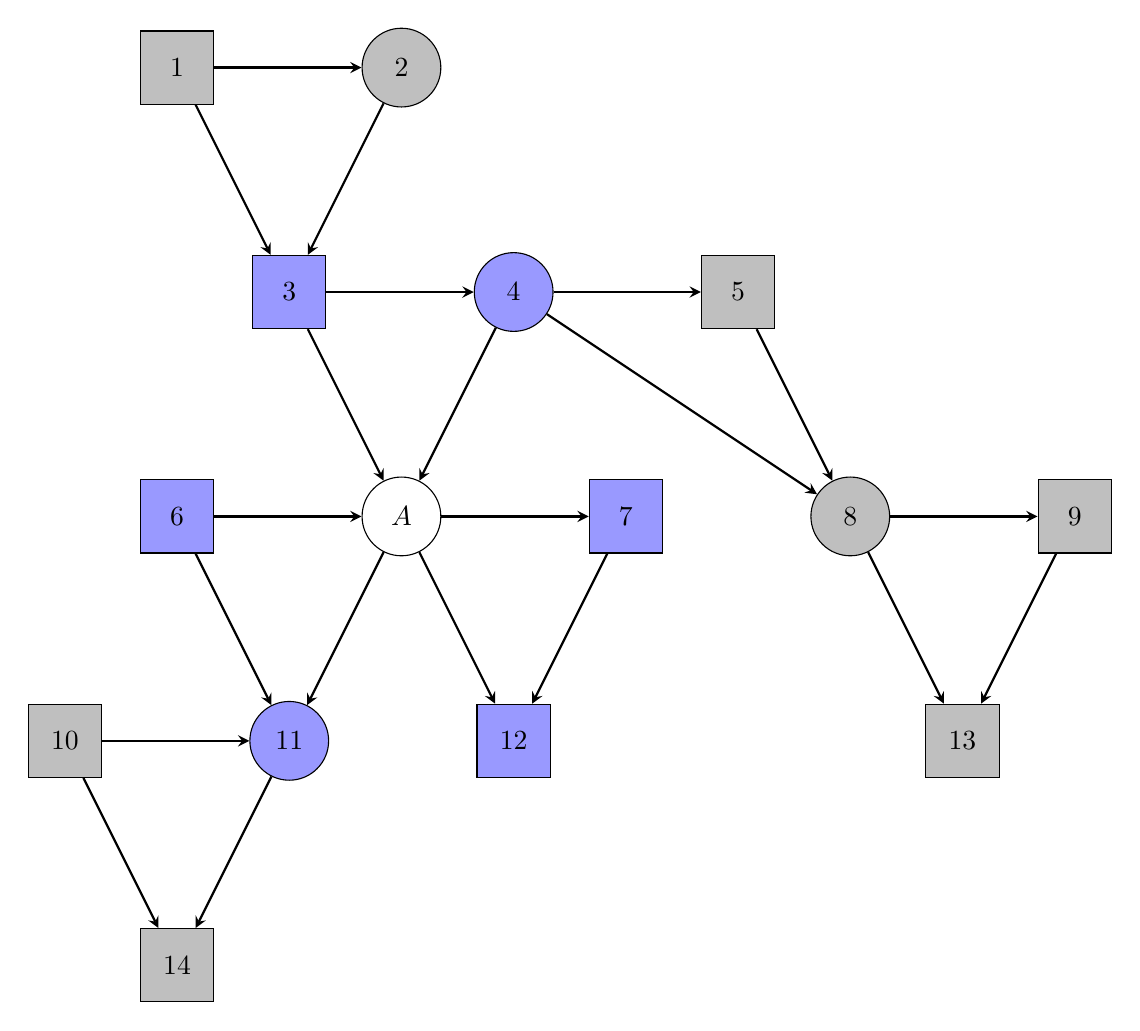
\begin{tikzpicture}[node distance=2.85cm]


\node (1) [opa] {1};
\node (2) [oma, right of=1] {2};

\node (3) [bpa, below of=1, xshift=1.425cm] {3};
\node (4) [bma, right of=3] {4};
\node (5) [opa, right of=4] {5};

\node (6) [bpa, below of=3, xshift=-1.425cm] {6};
\node (A) [ma, right of=6] {$A$};
\node (7) [bpa, right of=A] {7};
\node (8) [oma, right of=7] {8};
\node (9) [opa, right of=8] {9};

\node (10) [opa, below of=6, xshift=-1.425cm] {10};
\node (11) [bma, right of=10] {11};
\node (12) [bpa, right of=11] {12};
\node (13) [opa, right of=12, xshift=2.85cm] {13};

\node (14) [opa, below of=10, xshift=1.425cm] {14};

\draw [arrow] (1) -- (3);
\draw [arrow] (2) -- (3);

\draw [arrow] (3) -- (A);
\draw [arrow] (4) -- (A);
\draw [arrow] (4) -- (8);
\draw [arrow] (5) -- (8);

\draw [arrow] (6) -- (11);
\draw [arrow] (A) -- (11);
\draw [arrow] (A) -- (12);
\draw [arrow] (7) -- (12);
\draw [arrow] (8) -- (13);
\draw [arrow] (9) -- (13);

\draw [arrow] (10) -- (14);
\draw [arrow] (11) -- (14);

\draw [arrow] (1) -- (2);
\draw [arrow] (3) -- (4);
\draw [arrow] (4) -- (5);
\draw [arrow] (6) -- (A);
\draw [arrow] (A) -- (7);
\draw [arrow] (8) -- (9);
\draw [arrow] (10) -- (11);

\end{tikzpicture}
\tikzstyle{arrow} = [thick,->,>=stealth]
\end{center}
Notice that in this graph, all the blue vertices are indeed adjacent to $A$.  
The neighbors of any vertex $V$ in an undirected graphical model are sometimes
called the {\em Markov blanket} of $V$. The adjacency properties of an undirected
graph determine a whole set of {\em Markov properties} that dictate {\em
conditional independence} relations between variables. $V$ is conditionally independent
of everything else in the graph given its Markov blanket.

\section{Undirected graphical models}
\subsection{Factorization}
Like DAGs, undirected graphical models represent factorizations of probability distributions
but do so in terms of a product of {\em potentials} over {\em cliques} rather than a product
over vertices of conditional probabilities.  Additionally, the joint probabilities represented
by undirected graphs are often unnormalized (\ie the normalizing constant is not known).
A joint probability on variables $Y_1, \ldots, Y_K$ that respect an undirected graph $G$
in which the vertices are $Y_1, \ldots, Y_K$ factorizes according to:
\[
P(Y_1, \ldots, Y_K) = \frac{1}{Z}\prod_{C\in \mathrm{cl}(G)}\psi_C(X_C)
\]
where $\mathrm{cl}(G)$ is the set of all cliques in $G$, $X_C$ is a subset of variables 
$Y_1, \ldots, Y_K$ that form the clique $C$, $\psi_C$ is a potential---a
nonnegative function defined on $X_C$---and $Z$ is a (possibly unknown) normalizing
constant. This also holds when $\mathrm{cl}(G)$ is the set
of all {\em maximal cliques}.  We will leave it to the reader (and it is fairly
clear) that since the cliques are Ma-Pa-Kid trios, the potentials can be defined to be
the conditional probablities as well as any priors on individuals that have no
parents in the pedigree, thus giving us the same factorization as we had with the
directed graph.

\subsection{Elimination algorithm, treewidth, etc.}
Undirected graphs play a useful role in understanding how computationally difficult
it might be to do exact inference for an unobserved vertex in a graph.  We won't 
be able to say much about that now, but for those interested, keywords are
{\em elimination algorithm}, {\em tree decomposition of a graph}, {\em chordal graphs},
{\em treewidth}, and {\em junction tree algorithm}.  

\section{Inference in the presence of latent variables}
A common problem in statistics involves the sitution where the joint probability of all the
observed data cannot be easily computed because some data are missing.  These are often
called {\em missing data} problems or {\em latent variable} problems, and they can 
be understood graphically merely by the presence of unobserved variables in the graph, that
lie between the observed variables and the one(s) you wish to make inference about.

To take a concrete example, let's go back to our directed graph with individual $A$, but consider
what happens when individuals in $A$'s Markov blanket are not actually observed.  Note that, now, 
$A$'s more distant relatives are no longer irrelevant in inferring $Y_A$!  The DAG is shown
below with $A$ highlighted in red.
\begin{center}
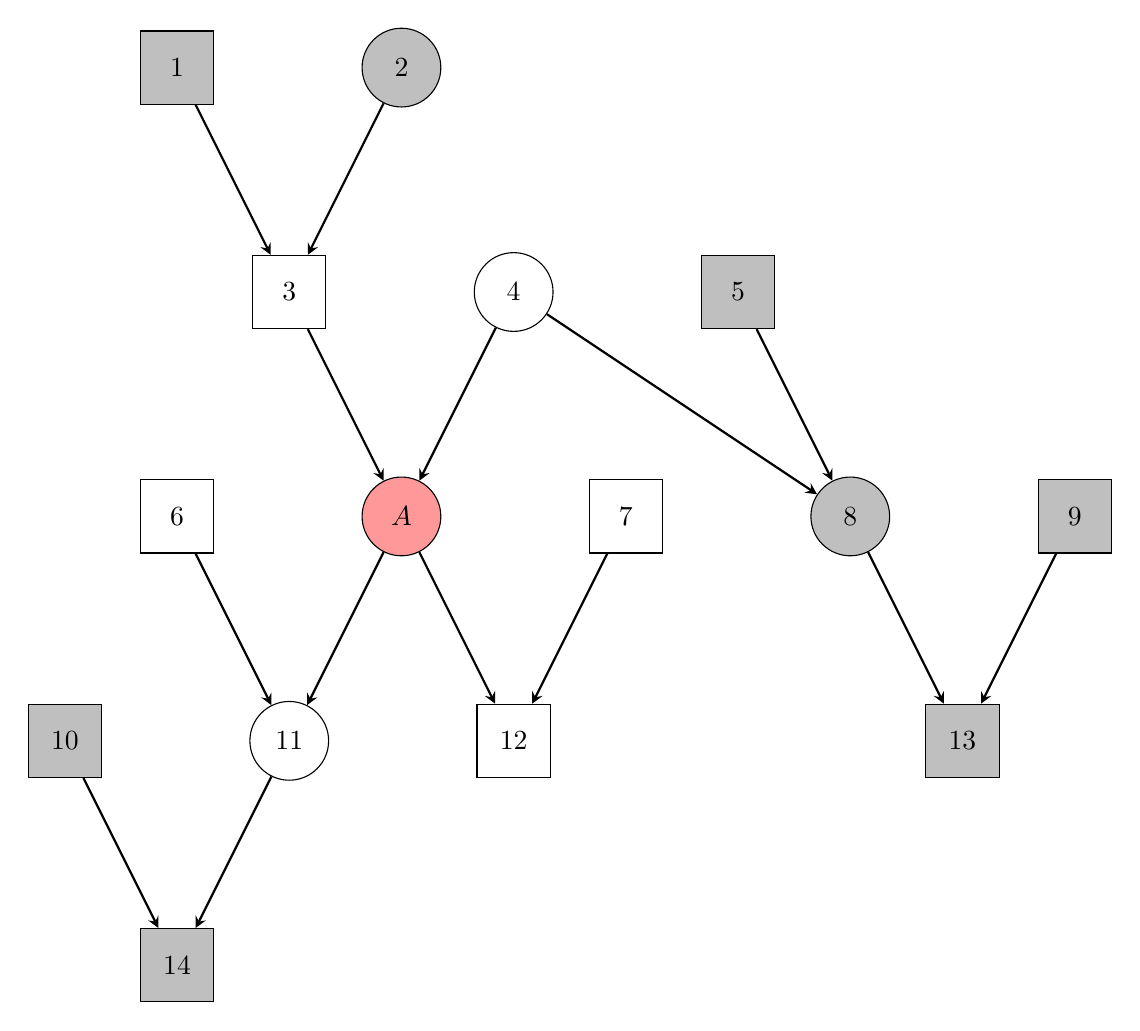
\begin{tikzpicture}[node distance=2.85cm]

\node (1) [opa] {1};
\node (2) [oma, right of=1] {2};

\node (3) [pa, below of=1, xshift=1.425cm] {3};
\node (4) [ma, right of=3] {4};
\node (5) [opa, right of=4] {5};

\node (6) [pa, below of=3, xshift=-1.425cm] {6};
\node (A) [rma, right of=6] {$A$};
\node (7) [pa, right of=A] {7};
\node (8) [oma, right of=7] {8};
\node (9) [opa, right of=8] {9};

\node (10) [opa, below of=6, xshift=-1.425cm] {10};
\node (11) [ma, right of=10] {11};
\node (12) [pa, right of=11] {12};
\node (13) [opa, right of=12, xshift=2.85cm] {13};

\node (14) [opa, below of=10, xshift=1.425cm] {14};

\draw [arrow] (1) -- (3);
\draw [arrow] (2) -- (3);

\draw [arrow] (3) -- (A);
\draw [arrow] (4) -- (A);
\draw [arrow] (4) -- (8);
\draw [arrow] (5) -- (8);

\draw [arrow] (6) -- (11);
\draw [arrow] (A) -- (11);
\draw [arrow] (A) -- (12);
\draw [arrow] (7) -- (12);
\draw [arrow] (8) -- (13);
\draw [arrow] (9) -- (13);

\draw [arrow] (10) -- (14);
\draw [arrow] (11) -- (14);

\end{tikzpicture}
\end{center}
Now, how do we do inference for $Y_A$, \ie how should we go about computing
\[
P(Y_A|Y_1, Y_2, Y_5, Y_8, Y_9, Y_{10}, Y_{13}, Y_{14})?
\]
The brute force method involves simply using the law of total probability [in other words, $P(A,B) = \sum_{C} P(A,B,C)$] to blindly sum the missing variables out of the joint distribution:
\[
\sum_{Y_3}\sum_{Y_4}\sum_{Y_6}\sum_{Y_7}\sum_{Y_{11}}\sum_{Y_{12}} P(Y_A, Y_1,\ldots,Y_{14})
\]
after which you can normalize that to sum to one over the three states $Y_A$ can take and Voila! you
have the conditional distribution you desire.  The brute force method, however,
is horribly inefficient, involving $3^6 = 729$ terms even though some parts of the sum don't
vary when other parts do owing to the way that $P(Y_A, Y_1,\ldots,Y_{14})$ factorizes.
Pursuing the brute force method would be akin to evaluating the sum
\[
\sum_{x=1}^{1000} \sum_{y=1}^{1000} f(x) g(y)
\]
by actually summing together 1,000,000 terms instead of noting that you could do it
by summing 2,000 terms along with one multiplication:
\[
\biggl(\sum_{x=1}^{1000} f(x)\biggr)
\biggl(\sum_{y=1}^{1000} g(y)\biggr)
\]

The key ingredient to figuring out how to do these types of sums efficiently
on joint probabilities is the factorization of the
joint probability. So, as you might expect, a graphical model interpretation can be useful
here. In fact, one of the clearest ways of expressing these types of operations relies
on another kind of graph that explicitly shows the factorization of a joint density 
(or any function).  This type of graph (last kind of graph for today\ldots I promise)
is called a {\em factor graph}.

\subsection{Factor graphs}
A factor graph is a {\em bipartite} graph with two classes of nodes: {\em variable nodes} which
represent variables (the same that vertices in a DAG do) and {\em factor nodes} which represent
functions.  

This type of graph forms the basis for the {\em sum-product algorithm}  and {\em belief propagation},
both loopy and otherwise.   From here on our we will be working from slides I made for a
separate talk on the topic.


\bibliography{anderson}
\bibliographystyle{mychicago}
\end{document}
